\documentclass[runningheads]{llncs}

\renewcommand{\labelenumii}{\theenumii}
\renewcommand{\theenumii}{\theenumi.\arabic{enumii}.}

\usepackage{graphicx}
\usepackage{hyperref} %might be better to uncomment this
\usepackage{subfig}
\usepackage{algpseudocode}
\usepackage{algorithm}

% Used for displaying a sample figure. If possible, figure files should
% be included in EPS format.
%
% If you use the hyperref package, please uncomment the following line
% to display URLs in blue roman font according to Springer's eBook style:
\renewcommand\UrlFont{\color{blue}\rmfamily}

\begin{document}
%
%\title{Contribution Title\thanks{Supported by organization x.}}
\title{[SCIR] Raport 2}
%
%\titlerunning{very very very }
% If the paper title is too long for the running head, you can set
% an abbreviated paper title here

\author{Bartłomiej Mastej}
%
%
\institute{Warsaw University of Technology, Warsaw, Poland}

%
\maketitle              % typeset the header of the contribution
%
%
%
%
\section{Konfiguracja węzła}
Wszelkie zmiany w projekcie są dostępne na GitHub'ie: \url{https://github.com/bartoszlomiej/weather-forecaster}.
Jako, że platformą uruchomieniową jest Rasbperry Pi 4 model B, zatem konfiguracja przesyłu danych poprzez WiFi nie była skomplikowana. Zostało to wskazane w raporcie 1.

Podsumowując:
\begin{enumerate}
\item Komunikacja Raspberry z chmurą oraz z komputerem odbywa się poprzez wbudowany moduł WiFi.
\item Komunikacja z komputerem odbywa sie poprzez protokuł $ssh$ do pełnej kontroli, oraz przez $scp$ do przesyłu plików.
\item Komunikacja z chmurą wykorzystuje protokół MQTT.
\item Chmura użyta w projekcie to $Thingspeak$.
\end{enumerate}

\section{Wstępna komunikacja z chmurą}
Do skonfigurowania połączenia z chmurą po stronie Raspberry Pi za pomocą protokołu MQTT została wykorzystana biblioteka $paho.mqtt$.
Za pomocą gotowego API należy wpisać wymagane dane - id kanału, dane uwierzytelniające klienta, port, nazwę hosta, socket.
Konfiguracja (bez danych uwierzytelniających - ze względów bezpieczeństwa) została zaprezentowana na Fig.~\ref{fig1}.
\begin{figure}
  %width=\textwidth
  \centering
  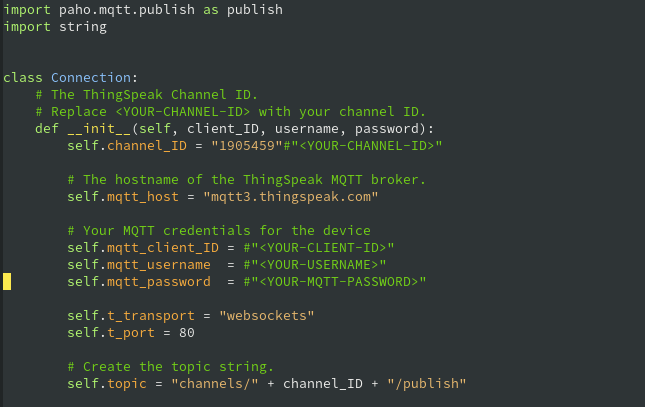
\includegraphics[width=\textwidth]{kod.png}
  \caption{Test odbierania danych w chmurze.} \label{fig1}    
\end{figure}

Wysyłanie danch z przygotowanym payload'em okazuje się bardzo proste - wystarczy użyć funkcji $publish$.

Po stronie chmury należy udostępnić <>. Na Fig.~\ref{fig2} zostało zaprezentowane prawidłowe odbieranie danych z raspberry pi. Jednakże, zamiast danych z czujników zostały wykorzystane parametry procesora (w celach testowych).
\begin{figure}
  %width=\textwidth
  \centering
  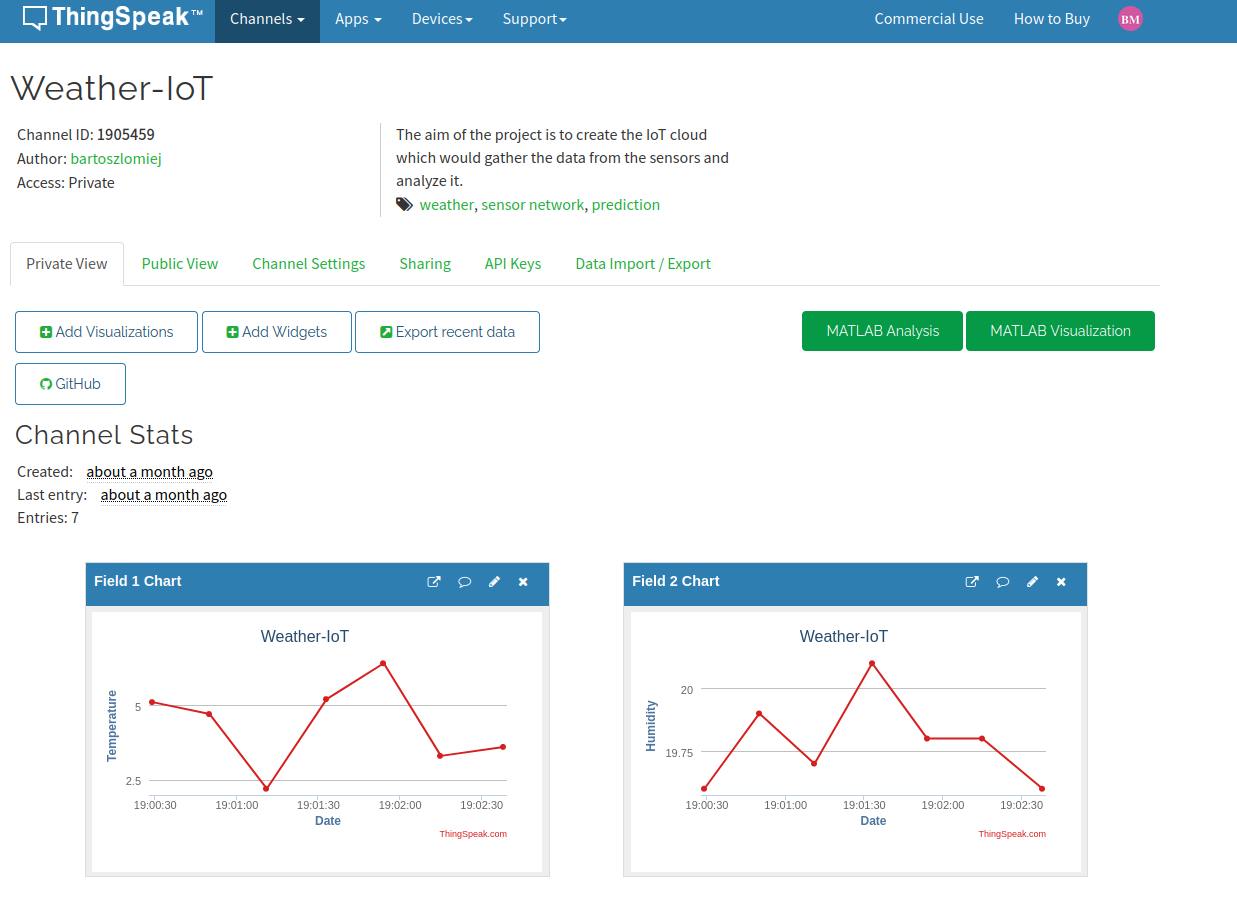
\includegraphics[width=\textwidth]{chumra.png}
  \caption{Test odbierania danych w chmurze.} \label{fig2}    
\end{figure}
\section{Parallelizm zbierania danych - multithreading}
W celu wykonywania pomiarów z czujnika jednocześnie został wprowadzony multithreading z wykorzystaniem biblioteki $threading$. Za jego pomocą każdy z czujników zbiera dane jednocześnie. Przed ich ujendoliceniem następuje synchronizaca wątków.

W przyszłości ma to na celu jednoczesne prztwarzania obrazu, zbierania danych z czujników jak i ich wysyłania jeśli chwilami będzie to konieczne. Jednakże, zostanie to rozważone ze względu na optymalizację poboru mocy.

\end{document}
